\documentclass[11pt]{article}
\usepackage[a4paper,margin=2.2cm]{geometry}
\usepackage[T1]{fontenc}
\usepackage{lmodern}
\usepackage{microtype}
\usepackage{amsmath,amssymb}
\usepackage{graphicx}
\usepackage{booktabs}
\usepackage{float}
\usepackage[font=small,labelfont=bf]{caption}
\usepackage[colorlinks=true,linkcolor=blue,citecolor=blue,urlcolor=blue]{hyperref}

\newcommand{\low}{\psi_{\mathrm{low}}}
\newcommand{\high}{\psi_{\mathrm{high}}}
\newcommand{\tile}[1]{\includegraphics[width=1.42cm]{figures/#1}}
\setlength{\parskip}{3pt}
\setlength{\textfloatsep}{12pt plus 2pt minus 2pt}
\setlength{\floatsep}{10pt plus 2pt minus 2pt}

\title{\vspace{-1.6cm}Which Frequencies Should Say ``Not a Cat''?\\[2pt]
\large Frequency-decoupled guidance, pushed the other way}
\author{Shahar Merom\\ \small Generative Learning and Diffusion Models, Technion, November 2026}
\date{}

\begin{document}
\maketitle
\vspace{-1.0cm}

\begin{abstract}
\noindent Frequency-decoupled guidance (FDG) gives the coarse and the fine part of an image their own guidance
strength. We test its claims on the pretrained EDM models for CIFAR-10, and then apply its split to negative
guidance (``generate anything except a cat''), which the paper does not study. Three things come out. First, the
split is a good tool for understanding guidance: on our model the low band's cost is the coarse layout, not the mean
colour, and the high band can change which class the image shows, so it is not just sharpening. Second, as a knob for
removing a class, the band split loses to a different idea: a strength that changes per image, as in the exact
``not $k$'' rule of Dynamic Negative Guidance. That rule removes half or more of the cats at an FID at or below that
of the unpushed model, and splitting it by band adds nothing. Third, timing matters more than the band: every push is cheap early and
expensive late, and pushing \emph{away} from a class acts earlier in sampling than pulling \emph{toward} one.
\end{abstract}

\section{Introduction}

Classifier-free guidance (CFG) makes a diffusion model follow its condition more closely, at the cost of variety
and, at high strength, of too strong colours. Sadat et al.\ \cite{fdg} look at CFG in the frequency domain. They
find that guiding the low frequencies causes the loss of variety and the colour problems, while guiding the high
frequencies improves detail. Their method, FDG, gives the two bands two different weights.

This report has two parts. In the first part (Section~\ref{sec:check}) we check FDG's main claims on a small model,
where we can afford many controlled runs. In the second part (Sections~\ref{sec:neg}--\ref{sec:pmap}) we ask a new
question: \emph{if we push away from a class, which band should do the pushing?} FDG only ever pulls toward a class,
and the paper never mentions negative guidance. A band split for ``not a cat'' could plausibly help: if the object
lives in the fine detail, a high-band push might remove the cat and leave everything else alone.

The two bands do remove a class in different ways, but no fixed split comes close to a rule whose strength depends
on the image. What matters most is \emph{when} we push and \emph{how hard for each image}, and the right time depends
on whether we push away from a class or toward one. Several of our predictions were wrong; we report those too.

\section{Background and definitions}
\label{sec:background}

\paragraph{Denoiser and sampler.} Let $x_0$ be a clean image and $x = x_0 + \sigma n$ a noisy copy, with
$n \sim \mathcal{N}(0, I)$; $\sigma$ is the \emph{noise level}. A diffusion model is a \emph{denoiser} $D(x;\sigma)$
trained to guess $x_0$ from $x$; the best guess is the average clean image given $x$, $\mathbb{E}[x_0 \mid x]$.
Tweedie's formula turns it into the score, $\nabla_x \log p(x;\sigma) = (D(x;\sigma) - x)/\sigma^2$. To generate,
we start from pure noise at $\sigma = 80$ and solve the probability-flow ODE $dx/d\sigma = (x - D(x;\sigma))/\sigma$
down to $\sigma = 0$. We use the EDM sampler \cite{edm}: 18 steps of Heun's method (Euler plus a correction), which
costs 35 denoiser calls. Any rule below only changes the $D$ that the sampler sees.

\paragraph{CFG.} A class-conditional denoiser $D_c$ is trained on images of class $c$, an unconditional one $D_u$ on
all images. CFG \cite{cfg} uses $D = D_u + w\,(D_c - D_u)$. Since
$\nabla \log p(c \mid x) = (D_c - D_u)/\sigma^2$ for ideal networks, CFG samples roughly from
$p(x)\,p(c\mid x)^w$: $w = 1$ is the conditional model, and $w > 1$ favours images that look clearly like $c$.

\paragraph{The band split and FDG.} We split any image-sized array $v$ into a low and a high band,
$v = \low[v] + \high[v]$. Our $\low$ keeps the Fourier coefficients below 4 cycles per image (radius
$r_c = 0.125$ cycles per pixel, with a soft sigmoid edge of width $0.02$), and $\high[v] = v - \low[v]$. At
$32\times32$ pixels the low band holds the mean colour, the large colour blobs and the rough layout; the high band holds
edges, outlines and texture (Figure~\ref{fig:tiles}a). FDG \cite{fdg} guides each band with its own weight:
\begin{equation}
  D = D_u + w_{\mathrm{low}}\, \low[D_c - D_u] + w_{\mathrm{high}}\, \high[D_c - D_u].
  \label{eq:fdg}
\end{equation}
We write an FDG setting as $(w_{\mathrm{low}}, w_{\mathrm{high}})$; $(w, w)$ is CFG. The paper uses a Laplacian
pyramid instead of our Fourier mask. On our model the two agree: FDG $(1,3)$ gives FID 6.07 with the mask and 6.31
with the pyramid (10k images each), a gap about twice the FID noise of such runs.

\begin{figure}[t]
  \centering
  \begin{minipage}[b]{0.335\textwidth}
    \centering\setlength{\tabcolsep}{1pt}
    \begin{tabular}{ccc}
      \tile{band_467_img.png} & \tile{band_467_low.png} & \tile{band_467_high.png} \\[-1pt]
      \tile{band_82_img.png} & \tile{band_82_low.png} & \tile{band_82_high.png} \\
      \scriptsize image & \scriptsize $\low[x]$ & \scriptsize $\high[x]$
    \end{tabular}\\[2pt]
    {\small (a) the band split}
  \end{minipage}\hfill
  \begin{minipage}[b]{0.64\textwidth}
    \centering\setlength{\tabcolsep}{1pt}
    \begin{tabular}{r@{\hspace{4pt}}ccc@{\hspace{5pt}}cc}
      \raisebox{0.6cm}{\scriptsize no push} & \tile{neg3_none_2.png} & \tile{neg3_none_21.png} & \tile{neg3_none_29.png} & \tile{neg3_none_11.png} & \tile{neg3_none_40.png} \\[-1pt]
      \raisebox{0.6cm}{\scriptsize low, $a=1$} & \tile{neg3_low1_2.png} & \tile{neg3_low1_21.png} & \tile{neg3_low1_29.png} & \tile{neg3_low1_11.png} & \tile{neg3_low1_40.png} \\[-1pt]
      \raisebox{0.6cm}{\scriptsize high, $b=2$} & \tile{neg3_high2_2.png} & \tile{neg3_high2_21.png} & \tile{neg3_high2_29.png} & \tile{neg3_high2_11.png} & \tile{neg3_high2_40.png}
    \end{tabular}\\[2pt]
    {\small (b) ``not a cat'', same noise in each column}
  \end{minipage}
  \caption{(a) A CIFAR-10 cat and car, their low band and their high band (shown around grey and stretched). (b) Without
  a push the first three images look like cats and the last two are horses. The low-band push often replaces the whole
  picture, even for the horses; the high-band push more often keeps layout and colours and changes the object.
  Hand-picked from the first 64 of 5,000 images.}
  \label{fig:tiles}
\end{figure}

\paragraph{Negative guidance.} To sample ``anything but class $k$'', the simple rule flips the sign,
$D = D_u - w\,(D_k - D_u)$. By the same argument it aims at $p(x) / p(k\mid x)^w$, which pushes \emph{every} image,
including ones that are clearly not of class $k$. Our question is what happens if we give this push one strength per band:
\begin{equation}
  D = D_u - a\, \low[D_k - D_u] - b\, \high[D_k - D_u].
  \label{eq:negband}
\end{equation}
Here $a$ is the low-band strength and $b$ the high-band strength. We call $D = D_u$ \emph{no push}.

\paragraph{The exact ``not $k$'' rule.} The images that are truly not class $k$ follow $p(x)(1 - p(k\mid x))$. Their
denoiser can be written with the same networks. For ideal networks, $D_u = \sum_j p(j\mid x)\, D_j$, because the
average clean image is the average over classes of each class's average. Removing class $k$ from this sum and
renormalising gives
\begin{equation}
  D_{\neg k} = \frac{D_u - p(k\mid x)\, D_k}{1 - p(k\mid x)} = D_u - \frac{p(k\mid x)}{1 - p(k\mid x)}\,(D_k - D_u).
  \label{eq:exact}
\end{equation}
So the exact rule is the sign flip with a strength $g = p/(1-p)$ that changes with the image and the noise level. This
rule is not ours: it is eq.~10 of Dynamic Negative Guidance (DNG) \cite{dng}, which adds an extra scale. We need
$p(k\mid x)$ at every step. We estimate it from the networks themselves: we run $D_j$ for all ten classes and find the
weights $p$ on the simplex that make $\sum_j p_j D_j$ closest to $D_u$ (a small least-squares fit). This costs 11
network calls per evaluation instead of 2. We cap $g$ at 20. We write $(\alpha, \beta)$ for the rule with
$g\,[\alpha\,\low + \beta\,\high]$; $(1,1)$ is eq.~\eqref{eq:exact}, the others are scaled versions of it.

\section{Setup}
\label{sec:setup}

\paragraph{Models.} All runs are inference only, with the public EDM checkpoints for CIFAR-10 \cite{edm}: a
class-conditional and a separately trained unconditional network (the ``VP'' pair, used everywhere unless stated). EDM
also released a second, independently trained pair (``VE''), which we use as a check. Images are $32\times32$.

\paragraph{Metrics.} \emph{FID} \cite{fid} compares the Inception features of generated and real images (lower is
better). For CFG runs the reference is the CIFAR-10 training set. For ``not $k$'' runs it is the 45,000 training
images of the other nine classes, so an image of class $k$ counts as wrong. FID depends on the number of generated
images, so we only compare FIDs at the same sample size. \emph{IS} \cite{is} (Inception score) rewards confident and
varied class predictions (higher is better). To read the class of each image we use two pretrained CIFAR-10
classifiers, ResNet-56 and VGG-16 \cite{chenyao}. \emph{Accuracy} is the share of guided images that ResNet-56
assigns to the requested class; \emph{cats left} is the share it calls cat. VGG-16 gives similar rates (within
0.6 points in every arm we report, except plain $D_c$ in Table~\ref{tab:pairs}: 1.2). Both classifiers mostly read the high band. For example, FDG $(3,1)$ guides only the low band;
its low band on top of the unguided high band gives accuracy 0.948 (0.951 at $w = 1$), while the unguided low band
with its high band gives 0.977. So we add a \emph{blurred reader} that cannot see the high band: it keeps only $\low[x]$, adds noise at $\sigma = 0.6$, and picks the class whose VE denoiser
prediction fits $\low[x]$ best (a diffusion classifier \cite{diffclf}). On 1,000 blurred real test images it is right
59\% of the time; it calls 50\% of real cats ``cat'' and 6.6\% of other images ``cat''. It reads the first 2,000
images of each run.

\paragraph{Pairing and side effects.} Every run uses the same noise for image $i$, so we can compare an image with
its unpushed twin. For ``not a cat'' we report: \emph{kept}, the share of images that are cats without a push and
still are; \emph{changed}, the share of the other images whose class changes; and \emph{dogs kept}, the share of
dogs (the most similar class) that stay dogs. \emph{Colour} is the shift of the mean colour along the direction
(cat mean colour $-$ global mean colour), in units of that difference.

\paragraph{Baselines.} \emph{No push} is $D_u$ alone, which gives about 9\% cats. The \emph{correct answer} is
the conditional network $D_c$ with labels spread evenly over the nine other classes. It is a reference, not a target
that pushing $D_u$ can reach: it uses a different network and has exactly the class mix of the FID reference.

\paragraph{Sample sizes and noise.} CFG runs use 10k images, ``not $k$'' runs 5k, unless stated. Runs were made on
two machines (an Azure A10 and a Colab A100). The same arm with the same noise differs by up to 0.35 FID between them
(no push: 7.61 and 7.72), because GPU arithmetic is not exactly repeatable, so we do not mix machines in one comparison
without saying so. Over three noise seeds, the main ``not a cat'' arms move by 0.1 to 0.9 FID and by up to 0.5
points of cats. Most other arms have one seed.

\section{Checking the paper}
\label{sec:check}

\paragraph{The big gain is mostly an equal-$w$ effect.} The paper's Table~1 compares CFG and FDG at the same $w$:
on EDM2-S, FID 9.77 for CFG at $w = 3$ against 5.44 for FDG. But its Fig.~5 (its only sweep; the model is unnamed but matches EDM2-S at $w = 3$) shows
CFG at $w = 1.5$ already near 5.45, and the best FDG setting near 5.0 (read from the plot). So best against best,
the gain is about 0.5 FID on that model. Our CIFAR-10 runs agree (Figure~\ref{fig:fidis}): at equal accuracy (0.985),
plain CFG at $w = 1.5$ has a better FID than FDG $(1,3)$ (4.87 against 6.07), while FDG has the higher IS (10.05
against 9.79). Guiding with CFG only for $\sigma \in [0.3, 2]$ (a guidance interval \cite{gi}) beats FDG $(1,3)$ in FID at
the same IS (5.22 against 6.07). The paper reports the opposite for SDXL in its Table~3, but with other models and metrics.

\begin{figure}[t]
  \centering
  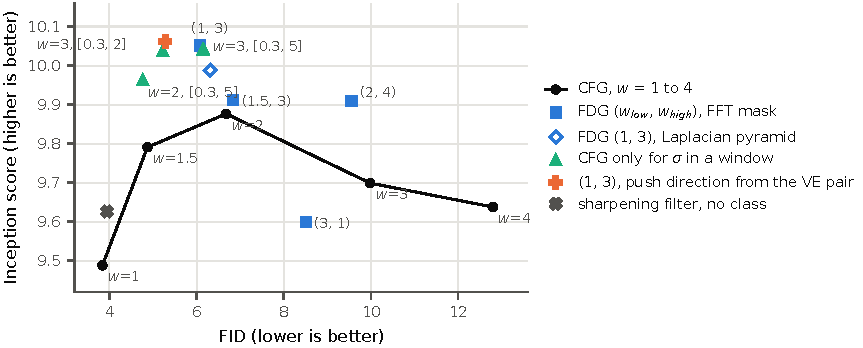
\includegraphics[width=0.86\textwidth]{figures/fid_is.pdf}
  \caption{Quality (IS) against fidelity (FID) on CIFAR-10, 10k images per point, one seed. FDG $(1,3)$ sits above the
  CFG curve, but at equal FID or equal accuracy plain CFG with a lower $w$ is close, and a time window or a push
  direction from the second network pair does as well with no band split. Noise: about 0.1--0.2 FID and 0.1 IS.}
  \label{fig:fidis}
\end{figure}

\paragraph{The low band's harm is the coarse layout, not the colour.} If the low band only shifted the colours,
freezing the mean colour (the zero-frequency or ``DC'' term) should remove most of its harm. We split the guidance
into three parts (mean colour, the rest of the low band, the high band), gave each a weight of 1 or 3, and ran all
eight combinations (Table~\ref{tab:dials}). Turning up the mean colour alone costs +1.07 FID, the rest of the low band
alone +3.52, and the high band alone +2.23. Averaged over the grid, the costs are 0.86, 3.43 and 1.90. So the layout
part costs far more than the colour, even though the colour shift itself comes almost only from the mean colour
(colour 1.09 against 0.09). The single-part costs sum to 6.82, against 6.14 for full $w = 3$, so they overlap a little.

\begin{table}[t]
  \centering
  \small
  \caption{Guiding three parts of the CFG signal separately, $w = 3$ or 1 for each (10k images, one seed). Precision
  and recall \cite{prc} measure quality and coverage of the real images. ``Colour'' is the shift of the mean colour
  toward the class mean colour, in units of (class mean $-$ global mean), against $w = 1$. ``Sharp'' is the rms of
  the high band relative to real images. The last three rows are high-band controls, each dosed to the same final
  sharpness as FDG $(1,3)$; $c'$ is a random wrong class.}
  \label{tab:dials}
  \begin{tabular}{lccccccc}
    \toprule
    Weights (mean colour, rest of low, high) & FID & IS & accuracy & precision & recall & colour & sharp \\
    \midrule
    (1, 1, 1) \; CFG $w=1$          & 3.84 & 9.49 & .951 & .670 & .656 & 0    & 1.03 \\
    (3, 1, 1) \; mean colour only   & 4.91 & 9.60 & .961 & .687 & .615 & 1.09 & 1.01 \\
    (1, 3, 1) \; rest of low only   & 7.36 & 9.66 & .991 & .702 & .591 & 0.09 & 1.05 \\
    (3, 3, 1) \; FDG $(3,1)$        & 8.50 & 9.60 & .990 & .710 & .558 & 1.10 & 1.03 \\
    (1, 1, 3) \; FDG $(1,3)$        & 6.07 & 10.05 & .985 & .535 & .720 & 0.01 & 1.15 \\
    (3, 1, 3)                       & 6.74 & 10.01 & .985 & .559 & .689 & 1.08 & 1.13 \\
    (1, 3, 3) \; mean colour frozen & 9.42 & 9.81 & .991 & .548 & .652 & 0.10 & 1.17 \\
    (3, 3, 3) \; CFG $w=3$          & 9.98 & 9.70 & .991 & .567 & .626 & 1.09 & 1.15 \\
    \midrule
    sharpening filter $\lambda(\sigma)\,\high[D_c]$, no class & 3.95 & 9.63 & .953 & .607 & .695 & 0 & 1.16 \\
    high band of $D_c - D_{c'}$                              & 11.30 & 10.28 & .988 & .576 & .695 & 0 & 1.16 \\
    high band of $D_{c'} - D_u$ (toward $c'$)                & 24.01 & 7.85 & .170 & .438 & .656 & 0 & 1.18 \\
    \bottomrule
  \end{tabular}
\end{table}

\paragraph{The high band is not just sharpening, and it can steer the class.} A sharpening filter tuned to FDG's
final sharpness leaves accuracy at the level of $w = 1$ (0.953 against FDG's 0.985) and costs almost no FID. So
FDG's high band carries class information, not only contrast. When we push only the high band toward a random wrong
class $c'$, 69\% of the images read as $c'$ (69\% for VGG-16 too; 0.5\% without the push), and objects visibly
change while layout and colours stay. Two caveats apply. The paper says the low band is the main driver of class
alignment (its Sec.~5.3), and on our model the low band also raises accuracy: low-only $(3,1)$ reaches 0.990 and
high-only $(1,3)$ 0.985, against 0.951 at $w = 1$. And our classifiers mostly read the high band, so class rates
favour high-band effects. The safe statement is that at $32 \times 32$ the high band alone \emph{can} steer the
class. One more difference from the paper: raising $w_{\mathrm{high}}$ lowers precision here (0.535 against 0.670),
while the paper reports that it improves precision.

\paragraph{Where the guidance signal is real.} $D_c - D_u$ mixes the class signal with the disagreement between two
separately trained networks. EDM's second pair (VE) gives an independent estimate; if each estimate is signal plus
independent error, the cosine between them measures the signal share. In the high band, the two pairs agree on the
true class at high noise (cosine 0.72--0.74 for $\sigma = 5$--13; $(1,3)$ path, $n = 256$) but not at low noise
(0.30 at $\sigma = 1.9$, 0.05 at 0.6). The networks still know the class there: toward a \emph{wrong} class they agree
(0.69 at $\sigma = 1.9$, 0.61 at 0.3; $w = 1$ path, $n = 256$). The true-class push is small at low noise because the
image already shows its class. Taking the FDG direction
from the VE pair, $D = D_c + 2\,\high[D_c^{\mathrm{VE}} - D_u^{\mathrm{VE}}]$ with the VP $D_c$ as the base, improves FDG $(1,3)$ from FID 6.07 to 5.28 at the same
IS. A related finding prepares the second part. Pushing the high band toward $c'$ in only one noise window gives
almost nothing for $\sigma \geq 3$ (0.5--0.7\% read as $c'$), 7.5\% for $\sigma \in [0.8, 3]$ and 55\% for
$\sigma < 0.8$ ($n = 2000$ each). So a push \emph{toward} a class in the high band works late in sampling.

\section{Main experiment: which band removes a class?}
\label{sec:neg}

We apply eq.~\eqref{eq:negband} with $k = $ cat and vary $a$ and $b$ (Table~\ref{tab:notcat},
Figure~\ref{fig:notcat}a). Our prediction was that the high band would win, because the classifiers and the
wrong-class push both point to the high band as the carrier of the object.

\begin{table}[t]
  \centering
  \small
  \caption{``Not a cat'', 5k images, one seed, Azure runs. Cats: ResNet-56; blurred: the low-band reader (2k images).
  FID against real non-cats. Kept, changed and dogs kept are paired with the no-push image of the same noise.
  ``Early'' is $\sigma \geq 0.8$ (11 of 18 steps), ``late'' is $\sigma < 0.8$.}
  \label{tab:notcat}
  \begin{tabular}{lrrrrrrr}
    \toprule
    Arm & cats left & blurred & FID & IS & kept & changed & dogs kept \\
    \midrule
    no push ($D_u$)                  & 9.0\% & 9.4\% & 7.61 & 9.12 & -- & -- & -- \\
    correct answer (reference)       & 1.5\% & 6.4\% & 6.42 & 9.21 & -- & -- & -- \\
    \midrule
    low $a = 0.5$                    & 3.3\% & 3.8\% & 10.43 & 8.46 & 32\% & 27\% & 50\% \\
    low $a = 1$                      & 1.2\% & 1.3\% & 19.24 & 7.91 & 11\% & 40\% & 31\% \\
    low $a = 2$                      & 0.2\% & 0.7\% & 39.53 & 6.57 & 2\% & 57\% & 11\% \\
    high $b = 0.5$                   & 5.6\% & 7.3\% & 8.71 & 9.30 & 61\% & 8\% & 85\% \\
    high $b = 1$                     & 3.9\% & 6.1\% & 12.97 & 9.21 & 42\% & 13\% & 78\% \\
    high $b = 2$                     & 2.1\% & 4.7\% & 22.09 & 9.02 & 23\% & 19\% & 63\% \\
    both $a = b = 0.5$               & 1.9\% & 3.1\% & 16.18 & 8.42 & 19\% & 29\% & 47\% \\
    both $a = b = 1$                 & 0.4\% & 1.2\% & 31.95 & 7.60 & 4\% & 42\% & 27\% \\
    \midrule
    low $a = 1$, early only          & 1.4\% & 2.1\% & 17.11 & 7.92 & 13\% & 40\% & 31\% \\
    low $a = 1$, late only           & 7.8\% & 7.3\% & 7.39 & 9.31 & 86\% & 2\% & 96\% \\
    high $b = 2$, early only         & 3.2\% & 5.1\% & 11.07 & 9.19 & 32\% & 18\% & 68\% \\
    high $b = 2$, late only          & 5.7\% & 8.2\% & 13.90 & 9.50 & 61\% & 6\% & 88\% \\
    \bottomrule
  \end{tabular}
\end{table}

\paragraph{The low band removes more cats at a lower FID.} This is against our prediction. At similar cat rates the
low band is cheaper: 3.3\% cats at FID 10.43 for $a = 0.5$ against 3.9\% at 12.97 for $b = 1$, and 1.2\% at 19.24 for
$a = 1$ against 2.1\% at 22.09 for $b = 2$. Pushing both bands lies about on the low-band curve. Two more noise seeds
(Colab) for five of the push points move them by at most 0.9 FID, most by less than 0.5, so the order holds. The
classifiers barely read the low band, yet they see the low band's effect: if we paste the unpushed low band back onto
the low-band-pushed images, they still read as cat only 1.6\% of the time. So an early push in the low band also
changes the final high band. Section~\ref{sec:pmap} measures this transfer directly.

\begin{figure}[t]
  \centering
  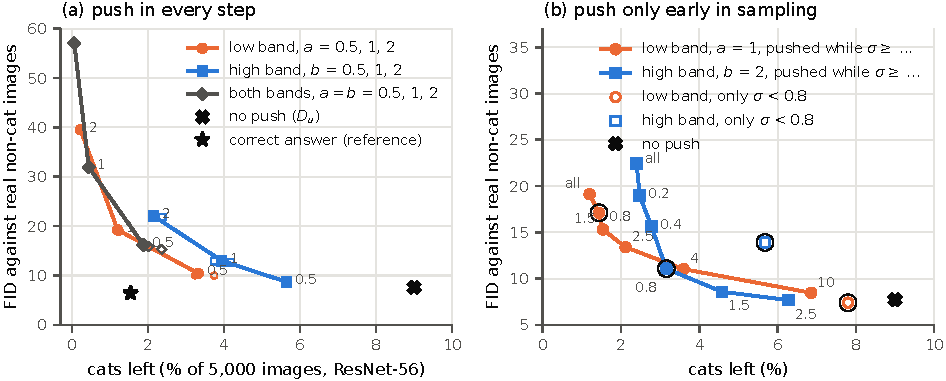
\includegraphics[width=\textwidth]{figures/notcat.pdf}
  \caption{``Not a cat'', 5k images. (a) Fixed pushes in every step (seed 0, Azure); the small open marks are seeds 1
  and 2 (Colab). (b) The same pushes applied only while $\sigma$ is above a threshold (the number next to each point),
  and $D_u$ after that. Points in (b) are Colab runs, except those with a black ring (Azure, same noise). The early part
  of each push removes most of the cats for a small part of the FID.}
  \label{fig:notcat}
\end{figure}

\paragraph{The two bands remove the class in different ways.} The low band moves images to a new picture, and this
hits everything. At $a = 1$ it changes the class of 40\% of the non-cat images, and only 31\% of dogs stay dogs. Removed
cats go to all classes almost evenly, and ships rise from 11\% to 18\% of all images. The mean colour also moves away
from cat colours (colour $-1.15$), and only about half of that ($-0.52$) is explained by the new class mix. The high
band keeps the picture and swaps the object. At $b = 2$ it changes 19\% of non-cats and keeps 63\% of dogs, and removed
cats most often become dogs (25\% of them). The colour hardly moves ($-0.05$). The cleanest comparison is at matched
removal: low $a = 0.5$ (3.3\% cats) changes 27\% of non-cats and keeps 50\% of dogs, while high $b = 1$ (3.9\%)
changes 13\% and keeps 78\%. So FID and the side effects disagree: the low band wins on FID, the high band on the class
mix. FID may not notice a changed class mix very well; we did not test this. ``Not a car'' gives the same picture
(5k, one seed): low $a = 1$ leaves 1.2\% cars at FID 16.58, high $b = 2$ leaves 5.1\% at 20.17. Under the high band the
removed cars most often become trucks or ships, while under the low band trucks fall from 10.4\% to 4.1\% of all images.

\paragraph{Timing: each push is cheap early and expensive late.} Figure~\ref{fig:notcat}b pushes only while $\sigma$
is above a threshold. The high band with $b = 2$, pushed only for $\sigma \geq 1.5$, leaves 4.6\% cats at FID 8.58;
the remaining steps remove 2.2 more points of cats for 13.9 more FID. The low band with $a = 1$, pushed only for
$\sigma \geq 2.5$, leaves 2.1\% at 13.39; going on to the end removes 0.9 more points for 5.7 more FID. Pushing only
late ($\sigma < 0.8$) does little: the low band removes almost nothing (7.8\% cats), the high band a bit at a high FID
cost. We predicted the low band would act early, which held. We also predicted the high band would act late, because
the toward-$c'$ push of Section~\ref{sec:check} did; that was wrong, and Section~\ref{sec:pmap} returns to it.

\paragraph{Two cheap tricks, and two that did not help.} Freezing the mean colour in the low band ($a = 1$ with the
DC term left alone) lowers FID from 19.11 to 16.01 at almost the same cat rate (1.2\% to 1.4\%), the colour shift
drops from $-1.15$ to $-0.18$, and the dogs are kept as before (33\% against 31\%). Pushing the high band only early is
the other trick: $b = 2$ for $\sigma \geq 0.8$ leaves 3.2\% cats at FID 11.07. Against low $a = 0.5$ (3.3\%, 10.43) its
FID is a little worse, but fewer non-cats change (18\% against 27\%) and more dogs stay (68\% against 50\%). Two ideas
gave nothing: taking the push direction from the VE pair (e.g.\ 3.3\% at 10.90 for the early high band), and pushing
each frequency only while the noise still hides it (1.1\% at 20.82, no better than the plain low band).

\begin{figure}[t]
  \centering
  \begin{minipage}[c]{0.5\textwidth}
    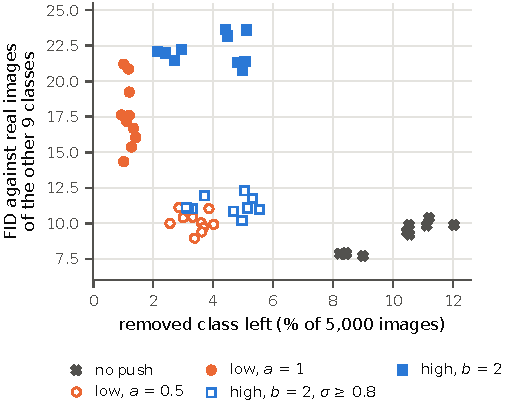
\includegraphics[width=\textwidth]{figures/classes.pdf}
  \end{minipage}\hfill
  \begin{minipage}[c]{0.47\textwidth}
    \captionof{figure}{All ten classes, each removed in turn (5k images, one seed each; cat from Azure, the rest
    Colab). The same pattern holds in every class: the low band at $a = 0.5$ leaves 2.6--4.0\% of the class at FID
    9.0--11.1, the full high band at $b = 2$ leaves 2.1--5.1\% at FID 20.8--23.7, and the early-only high band brings
    FID down to 10.2--12.3. No-push FIDs differ by class because the reference set changes; for five classes, low
    $a = 0.5$ has an FID at or below no push, since removing class $k$ itself improves the match.}
    \label{fig:classes}
  \end{minipage}
\end{figure}

\paragraph{All ten classes.} Figure~\ref{fig:classes} repeats the main arms for every class. Across classes, low $a = 1$
changes 37--49\% of the other images and keeps 18--56\% of the most similar class, while high $b = 2$ changes 19--25\%
and keeps 53--85\%. The high band removes some classes less well: 4.4--5.1\% are left for plane, car, frog, horse, ship
and truck, against 2.1--2.9\% for bird, cat, deer and dog.

\paragraph{``A dog, not a cat''.} With a target class, the usual way to add a negative prompt is FDG with $D_k$ in place
of $D_u$ (this is what the diffusers library does \cite{diffusers}): $D = D_k + w_{\mathrm{low}} \low[D_c - D_k] +
w_{\mathrm{high}} \high[D_c - D_k]$. Table~\ref{tab:pairs} shows three pairs, one seed each, with FID against real
images of the target class. For ``dog, not cat'' the high band wins: $(1,2)$ leaves 0.5\% cats at the FID of plain CFG
at $w = 2$, which leaves 1.9\%. For ``cat, not dog'' the arms lie on one trade-off curve. For ``truck, not car'' the
low band $(2,1)$ has the best FID, but only 0 to 6 cars are left in 5,000 images in the guided arms, so only FID
separates them. Which band is best depends on the pair. We do not use the blurred reader here: plain CFG toward dog
already reads 10.3\% ``cat'', and we have no rate for real dogs.

\begin{table}[t]
  \centering
  \small
  \caption{``$c$, not $k$'': class $k$ left (ResNet-56) / FID against real images of class $c$. 5k images, one seed
  (Colab). Plain $D_c$ is $(1,1)$. CFG uses $D_u$ as the base; the other arms use $D_k$.}
  \label{tab:pairs}
  \begin{tabular}{lccccc}
    \toprule
    Pair & plain $D_c$ & CFG $w = 2$ & high $(1,2)$ & low $(2,1)$ & both $(2,2)$ \\
    \midrule
    dog, not cat   & 7.72\% / 12.17 & 1.94\% / 15.18 & 0.48\% / 15.21 & 1.94\% / 16.93 & 0.20\% / 27.22 \\
    cat, not dog   & 5.08\% / 12.63 & 1.30\% / 18.56 & 0.44\% / 21.31 & 1.58\% / 17.92 & 0.10\% / 33.14 \\
    truck, not car & 1.08\% / 6.63  & 0.12\% / 11.70 & 0.04\% / 12.40 & 0.06\% / 10.50 & 0.00\% / 18.19 \\
    \bottomrule
  \end{tabular}
\end{table}

\section{The exact rule: strength per image, not per band}
\label{sec:exact}

No fixed push in Figure~\ref{fig:notcat} gets near the correct answer: near its cat rate (1.5\%), fixed and windowed
pushes cost FID 15--22 against 6.42. The exact rule, eq.~\eqref{eq:exact}, explains why. Its strength $p/(1-p)$ is
small for most images (0.03--0.2 on average during sampling), so it pushes the few images that are becoming cats and
leaves the rest alone.

\paragraph{It removes cats almost for free.} With 5k images (Figure~\ref{fig:exact}a), the exact rule $(1,1)$ leaves
4.2\% cats at FID 7.02, \emph{below} no push (7.72). The fixed pushes run on the same machine need FID 10.6--22.4 for
1.2--3.4\% cats, and every fixed or windowed push we ran has a higher FID than the exact rule at a similar cat rate. Three
noise seeds give 4.2/4.2/3.7\% cats at FID 7.02/6.81/6.71, against no push at 9.0/9.2/9.4\% and 7.72/7.77/7.66. Scaling
the rule up removes more cats along one curve: $(1.5,1.5)$ 2.6\% at 7.16, $(2,2)$ 1.8\% at 7.58 (only just below the
no-push values of 7.66--7.77). The side effects are small too (Table~\ref{tab:collateral}): $(1,1)$ changes only 11\% of
non-cats and keeps about 70\% of dogs.

\paragraph{Splitting it by band adds nothing.} Doubling one band lands on the same curve: $(2,1)$ gives 2.3\% at 7.40
(the curve is at about 7.33 there) and $(1,2)$ gives 3.0\% at 6.95 (curve about 7.13). Both differences are within the
seed noise. Fitting $p$ on one band only, or on each band for its own push, also changes nothing (4.0--4.4\% cats,
FID 6.98--7.04). A diagnostic explains this. We fitted $p$ on 2,000 unpushed paths and asked how well it predicts the
final class. For $\sigma$ between 13 and 58, only the low band carries some information (AUC for ``will be a cat''
0.60--0.65, against 0.51--0.55 for the high band); from $\sigma \approx 5$ down, the low band, the high band and the
whole image agree within 0.05 (AUC 0.76--0.96). So a separate posterior per band has little to add.

\begin{figure}[t]
  \centering
  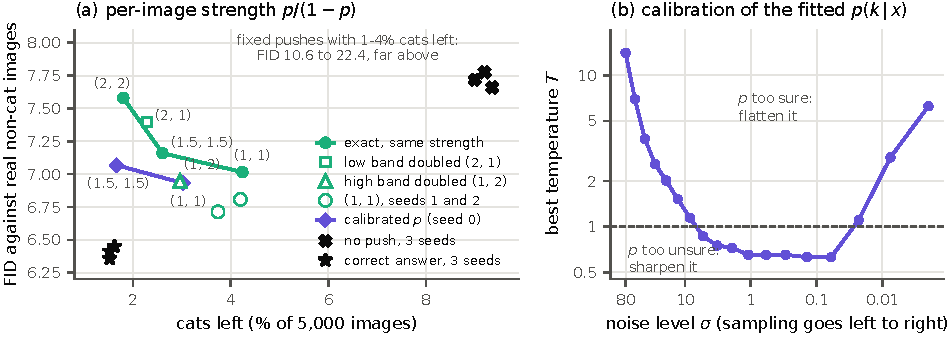
\includegraphics[width=\textwidth]{figures/exact.pdf}
  \caption{(a) The exact rule and its scaled versions, 5k images (Colab). All exact arms lie on or below one curve,
  well below the fixed pushes. The calibrated points use temperatures fitted on 2,000 no-push paths of the same noise
  seed, so they are optimistic. (b) The temperature $T$ that best calibrates the fitted $p(k\mid x)$ against the final
  class, $p \leftarrow \mathrm{softmax}(\log(p + 10^{-3})/T)$: the fit is too sure at high noise and too unsure at low
  noise.}
  \label{fig:exact}
\end{figure}

\paragraph{The fitted $p$ is badly calibrated, and fixing it helps.} The same diagnostic shows that the fitted
$p(k\mid x)$ is too sure at high noise: at $\sigma = 80$ its top class is right only 10\% of the time (chance), yet its
values are far from flat, and its average for cat swings from 3\% there to 13--16\% at $\sigma = 13$--28, while
9.8\% of these images end up as cats. At low noise it is too unsure: for $\sigma$ between 0.06
and 1.1 its top class is right 85--90\% of the time, but it gives the final class only 0.62--0.68 on average. A
temperature per noise level fixes this (Figure~\ref{fig:exact}b; $T = 14$ at $\sigma = 80$, about 2 at 19, 0.65 at
0.3--1.1). With the calibrated $p$, $(1,1)$ leaves 3.0\% cats at FID 6.93 and $(1.5,1.5)$ 1.7\% at 7.07, close to the
correct answer's cat rate (1.5\%). The second point is about 0.6 below the uncalibrated curve (extended to that cat rate). It also keeps fewer
cats as cats (16\% against 25\%) at the same side effects (Table~\ref{tab:collateral}). This result has one seed, and the
temperatures were fitted on the same noise, so it needs a held-out check.

\begin{table}[t]
  \centering
  \small
  \caption{Side effects of pushes that leave 1.7--4.0\% cats, paired by noise with no push. Fixed pushes: Azure, seed 0.
  Exact rule: Colab; $(1,1)$ is the mean of seeds 1 and 2; ``per band'' fits $p$ separately for each band's push.}
  \label{tab:collateral}
  \begin{tabular}{lccccc}
    \toprule
    Arm (5k images) & cats left & FID & cats kept & non-cats changed & dogs kept \\
    \midrule
    low $a = 0.5$                    & 3.3\% & 10.43 & 32\% & 27\% & 50\% \\
    high $b = 1$                     & 3.9\% & 12.97 & 42\% & 13\% & 78\% \\
    high $b = 2$, early only         & 3.2\% & 11.07 & 32\% & 18\% & 68\% \\
    exact $(1,1)$                    & 4.0\% & 6.76  & 38\% & 11\% & 71\% \\
    exact $(1,1)$, calibrated        & 3.0\% & 6.93  & 29\% & 10\% & 71\% \\
    exact $(1.5,1.5)$, per band      & 2.7\% & 7.18  & 25\% & 14\% & 63\% \\
    exact $(1.5,1.5)$, calibrated    & 1.7\% & 7.07  & 16\% & 13\% & 63\% \\
    \bottomrule
  \end{tabular}
\end{table}

\section{The push map: away acts earlier than toward}
\label{sec:pmap}

Two timing results seem to clash. Pushing the high band \emph{toward} a wrong class works late
(Section~\ref{sec:check}), but pushing the high band \emph{away} from cats works better early (Section~\ref{sec:neg}).
The two runs also had different base paths ($D_c$ and $D_u$). To compare fairly, we start 4,000 images on the
unguided path ($D_u$), push one band for just two sampler steps with strength 2, and then sample to the end with
$D_u$. ``Away'' pushes from the class the image would have become without a push; ``toward'' pushes to one other
class, chosen per image. We read the result with ResNet-56. The two directions need two measures. For ``away'' we
count any class change. For ``toward'' we report both the share that reached the target and the share whose class
changed at all.

\begin{figure}[t]
  \centering
  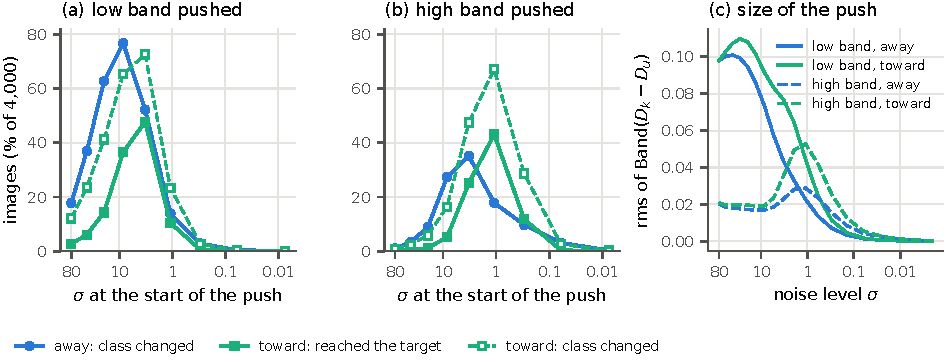
\includegraphics[width=\textwidth]{figures/pmap.pdf}
  \caption{The push map, 4,000 images, strength 2, one seed. Each point pushes one band for two steps starting at the
  given $\sigma$, on the unguided path, and then samples with $D_u$. (a, b) Away (any class change) peaks earlier than
  toward, by either toward measure. (c) The size of the push in each step: away and toward are about equal at high
  noise, but late in sampling the away push is only half to two thirds as large.}
  \label{fig:pmap}
\end{figure}

\paragraph{Result.} In both bands the away curve peaks earlier than the toward curves (Figure~\ref{fig:pmap}). In the
low band, away changes 77\% of images when pushed at $\sigma = 8.4$--5.3 and already 18\% at $\sigma = 80$--58, while
toward peaks at $\sigma = 3.3$--1.9 (48\% reach the target, 73\% change class). In the high band, away peaks at
$\sigma = 3.3$--1.9 (35\%), toward at $\sigma = 1.1$--0.6 (43\% reach the target, 67\% change). So by the same
measure (any change) toward is not weaker, but its peak is later.

Three things limit this result. First, the push sizes differ (Figure~\ref{fig:pmap}c). For $\sigma \geq 40$ they are
about equal, but later the away push is smaller (0.5--0.65 times the toward push for $\sigma \leq 3.3$), so a late
away push is simply weaker. At
$\sigma = 8.4$--5.3, though, the toward push is the larger one and still changes fewer images (65\% against 77\%).
Second, strength matters. At strength 1 the away peaks stay where they were (low band 56\% at $\sigma = 8.4$; high band
23\% at 3.3), but the low-band toward curve becomes flat (15.4\% at $\sigma = 8.4$ and 15.9\% at 3.3); VGG-16 finds the same peaks
there (within 0.03). Third, on a
Gaussian-mixture toy with exact denoisers ($n = 1000$) the shift in the low band is within noise, so we cannot say it
comes from the data alone. Our guess for the mechanism: to leave a class, an image only has to stop looking like it,
which the coarse layout can decide early; to reach a class, it has to beat all nine others, which needs the details.
We did not test this.

\paragraph{Band transfer.} The push map also shows why a low-band push changes what the classifiers see. A low-band
away push at $\sigma = 8.4$--5.3 changes the final high band by 0.72 times as much as the final low band (rms). A
high-band push at $\sigma = 3.3$--1.9 changes the final low band by 0.54 times its high-band change. So a band split of
the push is not a split of the result: what is pushed early in one band spreads to the other.

\section{Limitations}
\label{sec:limits}

Everything is on one small model (CIFAR-10 at $32 \times 32$, where our 4-cycle cut puts object outlines into the
high band), so results may differ at the paper's resolutions. Our check of the paper's equal-$w$ claim rests on its only sweep
(EDM2-S). The classifiers mostly read the high band; the blurred reader sees the low band but reads only 2,000 images,
calls 6.6\% of real non-cats ``cat'', and was never tested on real dogs, so we do not use it to rank the bands. FID is
measured at 5k images against a reference that excludes the removed class, so removing that class lowers FID by
itself. Most arms have one seed. The ten classes, the pairs, and the calibrated rule have one seed each, and the
calibrated rule was fitted on the same noise. Runs come from two machines that differ by up to 0.35 FID. The fitted
$p(k\mid x)$ is not a true posterior, and the exact rule needs 11 network calls per evaluation, 5.5 times plain
guidance. The images in Figure~\ref{fig:tiles} are hand-picked.

\section{Related work}
\label{sec:related}

DNG \cite{dng} introduced the per-image strength of eq.~\eqref{eq:exact}, and its MNIST experiment already shows
that removing a class changes how often the similar classes appear. ContrastiveCFG \cite{ccfg} also reshapes the negative push. Ban et al.\ \cite{ban} study
when a negative prompt acts in text-to-image models and report a delayed effect; they cancel a positive prompt, a
different setting from our ``away'' push, and our results suggest that an early negative push mainly acts through the
low band. Recent work calibrates a concept-presence gate for negative guidance \cite{crg}, steers away from a class with
sequential Monte Carlo \cite{smc}, composes models exactly with logical operations \cite{logdiff}, and calibrates noisy
classifiers for guidance \cite{calib}. Our checks of FDG relate to the guidance interval \cite{gi}, autoguidance
\cite{autoguidance}, and studies of CFG over time \cite{stagewise} and in linear models \cite{liwangqu}. In short searches we did not find a band split of the negative term, a band-by-time map of pushes toward
and away, or a per-noise calibration of the posterior used in guidance. Not finding them is weak evidence.

\section{Conclusion}
\label{sec:conclusion}

The frequency split is a useful lens on guidance, but not a better knob for removing a class.
A strength per image does that at no FID cost, the time of the push matters more than its band, and pushing away from
a class acts earlier than pulling toward one.

\begin{thebibliography}{99}
\small
\setlength{\itemsep}{1pt}
\bibitem{fdg} S.~Sadat, T.~Vontobel, F.~Salehi, R.~M.~Weber. Guidance in the Frequency Domain Enables High-Fidelity
  Sampling at Low CFG Scales. arXiv:2506.19713, 2025.
\bibitem{cfg} J.~Ho, T.~Salimans. Classifier-Free Diffusion Guidance. arXiv:2207.12598, 2022.
\bibitem{edm} T.~Karras, M.~Aittala, T.~Aila, S.~Laine. Elucidating the Design Space of Diffusion-Based Generative
  Models. NeurIPS 2022. arXiv:2206.00364.
\bibitem{dng} F.~Koulischer, J.~Deleu, G.~Raya, T.~Demeester, L.~Ambrogioni. Dynamic Negative Guidance of Diffusion
  Models. ICLR 2025. arXiv:2410.14398.
\bibitem{ban} Y.~Ban, R.~Wang, T.~Zhou, M.~Cheng, B.~Gong, C.-J.~Hsieh. Understanding the Impact of Negative Prompts:
  When and How Do They Take Effect? arXiv:2406.02965, 2024.
\bibitem{ccfg} J.~Chang, C.~Lee, H.~Chung, J.~C.~Ye. ContrastiveCFG: Guiding Diffusion Sampling by Contrasting
  Positive and Negative Concepts. arXiv:2411.17077, 2024.
\bibitem{gi} T.~Kynk\"a\"anniemi, M.~Aittala, T.~Karras, S.~Laine, T.~Aila, J.~Lehtinen. Applying Guidance in a
  Limited Interval Improves Sample and Distribution Quality in Diffusion Models. NeurIPS 2024. arXiv:2404.07724.
\bibitem{autoguidance} T.~Karras, M.~Aittala, T.~Kynk\"a\"anniemi, J.~Lehtinen, T.~Aila, S.~Laine. Guiding a
  Diffusion Model with a Bad Version of Itself. NeurIPS 2024. arXiv:2406.02507.
\bibitem{stagewise} C.~Jin, Q.~Shi, Y.~Gu. Stage-wise Dynamics of Classifier-Free Guidance in Diffusion Models.
  arXiv:2509.22007, 2025.
\bibitem{liwangqu} X.~Li, R.~Wang, Q.~Qu. Towards Understanding the Mechanisms of Classifier-Free Guidance.
  arXiv:2505.19210, 2025.
\bibitem{crg} Y.~Choi, C.~Oh, H.~Choi, S.~Seo, K.~Kim. Concept Removal Guidance: Evidence-Calibrated Negative
  Guidance for Safe Diffusion Sampling. arXiv:2606.29801, 2026.
\bibitem{smc} L.~Wang, L.~Ma, H.~St\"ark, R.~Barzilay. Specificity-Aware Diffusion Steering via Variance-Reduced
  Sequential Monte Carlo. arXiv:2610.00395, 2026.
\bibitem{logdiff} F.~Alesiani, J.~Warrell, T.~Bien, H.~Christiansen, M.~Ferraz, M.~Niepert. Logical Guidance for the
  Exact Composition of Diffusion Models. arXiv:2602.05549, 2026.
\bibitem{calib} S.~Javid, A.~Bagheri, N.~Gonz\'alez-Prelcic. Enhancing Diffusion Model Guidance through Calibration
  and Regularization. arXiv:2511.05844, 2025.
\bibitem{diffclf} A.~C.~Li, M.~Prabhudesai, S.~Duggal, E.~Brown, D.~Pathak. Your Diffusion Model is Secretly a
  Zero-Shot Classifier. ICCV 2023. arXiv:2303.16203.
\bibitem{fid} M.~Heusel, H.~Ramsauer, T.~Unterthiner, B.~Nessler, S.~Hochreiter. GANs Trained by a Two Time-Scale
  Update Rule Converge to a Local Nash Equilibrium. NeurIPS 2017.
\bibitem{prc} T.~Kynk\"a\"anniemi, T.~Karras, S.~Laine, J.~Lehtinen, T.~Aila. Improved Precision and Recall Metric
  for Assessing Generative Models. NeurIPS 2019.
\bibitem{is} T.~Salimans, I.~Goodfellow, W.~Zaremba, V.~Cheung, A.~Radford, X.~Chen. Improved Techniques for
  Training GANs. NeurIPS 2016.
\bibitem{chenyao} Y.~Chen. Pretrained CIFAR-10 models (ResNet-56, VGG-16-BN).
  \url{https://github.com/chenyaofo/pytorch-cifar-models}.
\bibitem{diffusers} P.~von Platen et al. Diffusers: State-of-the-art Diffusion Models.
  \url{https://github.com/huggingface/diffusers}, 2022.
\end{thebibliography}

\end{document}
